\documentclass[12pt,oneandhalf,chaparabic,ceng,ms,eng,oneside,pntc]{gsufbe}
% for Computer Engineering use option ceng
% for Industrial Engineeering use option ie
% for Logistics and Finance Management use option lfm
% for Mathematics use option math
% for MSc use option ms
% for PhD use option phd
% Don't change other options due to instutional regulations. 
% You can delete next line If your thesis does not have an appendix
\usepackage{appendix}

% Use your latex packages here
%\usepackage{indentfirst}
\usepackage{graphicx}
\usepackage{amsmath}
\usepackage{amsfonts}
\usepackage{amssymb}
\usepackage{enumitem}
\usepackage{amsthm}
\usepackage{subcaption}
\usepackage{booktabs}
\usepackage{array}
\usepackage[round]{natbib}
\usepackage{har2nat}
\usepackage{algorithmic}
\usepackage[ruled,noline]{algorithm2e}
\usepackage{titlesec}
\usepackage[section]{placeins}
\usepackage{float}

% End of Latex Packages
%
% Any personal Latex definition, decleration, etc.
\makeatletter
\let\old@includegraphics\includegraphics
\renewcommand{\includegraphics}[2][,]{%
  \setbox9=\hbox{\old@includegraphics[#1]{#2}}%
  \ifdim\wd9>\textwidth
    \old@includegraphics[#1,width=\textwidth]{#2}%
  \else
    \old@includegraphics[#1]{#2}%
  \fi%
}
\makeatother

% End of personal stuff
%
% Personal Information
% ----------------------------
%
% Please check this part and fill in information about your thesis
%
% Name and Surname
\author{Uğurcan Ergün}
% Thesis Title English and Turkish
\title{Evaluating Feasibility of Container Virtualization for Network Function Virtualization}
\trtitle{Ağ İşlevi Sanallaştırma için Konteynır Sanallaştırmanın Uygunluğunun İncelenmesi}
% Department : English and Turkish
%
% The departments are pre-defined, you need not redeclare them. 
% Date : You should indicate the month of your thesis defence in English.
% Default is this month
%
\date{June 2018}
%
% Approval Page Details
% --------------------------
% For each command you can give the title as optional parameter enclosed in [ ]
%For white covered thesis, please comment out approval page in cls file.
%Committee members number:
%-------------------
%Single advisor/masters thesis: 2 members excluding advisor
%Two advisors/master thesis: 3 members excluding both advisors
%Single advisor/PhD Thesis: 4 members excluding advisor
%Two advisors/PhD Thesis: 5 members excluding advisor
%Please comment out extra member of committee. 
%
% prof : Prof. Dr.
% assocprof : Assoc. Prof. Dr.
% assistprof : Assist. Prof. Dr.
% dr : Dr.
%
% Supervisor
\supervisor[assistprof]{B. ATAY ÖZGÖVDE}
\departmentofsupervisor{Computer Engineering Department, GSU}
% co-Supervisor

%\cosupervisor[assocprof]{JANE DOE}
%\departmentofcosupervisor{Management, UCL}
% Ask your supervisor if you are not sure
\committeememberi[assistprof]{}
\affiliationi{}
\committeememberii[assistprof]{}
\affiliationii{}
%\committeememberiii[assistprof]{ATAY ÖZGÖVDE}
%\affiliationiii{Computer Engineering Department, GSU}
% Fourth committee member
%\committeememberiv[assocprof]{MAN DOE}
%\affiliationiv{Computer Engineering Department, MIT}
% Fifth committee member
%\committeememberv[assistprof]{WOMAN DOE}
%\affiliationv{Computer Engineering Department, TOBB ETÜ}
%
% Keywords : English & Turkish & French, Comma seperated No more than 5 keywords
\keywords{}
\motscles{}
\anahtarklm{}
%
% Abstract in English
%
\abstract{
In modern computing it has become common practice to run software on virtual environments and commodity
hardware rather than specialized devices. But most of the network appliances in use are still propriety
hardware. There is a significant amount of work in the network function virtualization domain to
actualize these network functions in a virtualized manner. In this work we evaluate if it’s feasible to
use virtual network functions in a virtualization technology that is recently gaining traction called
operating system level virtualization or container virtualization. We examined if the necessary
technologies for virtual network function exists in container domain and ran experiments on prevalent
container platform Kubernetes to see if these platforms can match the requirements for the network 
functions.}

%
% Abstract in French
\resume{}
% Turkish Abstract
%
\oz{}
%
% Acknowledgements
\acknowledgments{}
%
% End of Personal and Introductory Information
%%%%%%%%%%%%%%%%%%%%%%%%%%%%%%%%%5
\setlength{\jot}{20pt}
%%% !!! This two should be last lines before \begin{document}, do no move them !!!
\usepackage[pdftex]{hyperref}
\usepackage[all]{hypcap}
\begin{document}
\addtolength{\textheight}{1.5cm}
% Preliminaries
\newlength\myindent
\setlength\myindent{6em}
\newcommand\bindent{%
  \begingroup
  \setlength{\itemindent}{\myindent}
  \addtolength{\algorithmicindent}{\myindent}
}
\newcommand\eindent{\endgroup}
\begin{preliminaries}
% If you are willing to use any custom stuff before Chapters, put it here
% Such as List of Abbreviations
% Check the abbreviations.tex for a template list of abbreviations
%\begin{theglossary}{TOSCA}
\item[API]   Application Programming Interface
\item[AUFS]  Advanced Multi-layered Unification File System
\item[BGP]   Border Gateway Protocol
\item[CAPEX] Capital Expenditures
\item[CDN]   Content Delivery Network
\item[CNI]   Container Network Interface
\item[CORD]  Central Office Re-architected as a Datacenter
\item[CPU]   Central Processing Unit
\item[CRI]   Container Runtime Interface
\item[ETSI]  European Telecommunications Standards Institute
\item[GiB]   Gigibyte
\item[HLC]   Home Location Register
\item[HSC]   Home Subscriber Server
\item[HTTP]  Hypertext Transfer Protocol
\item[JSON]  Javascript Object Notation
\item[I/O]   Input and Output
\item[IP]    Internet Protocol
\item[KVM]   Kernel Virtual Machine
\item[LXC]   Linux Containers
\item[MANO]  Management and Orchestration
\item[NAT]   Network Address Translation
\item[NFV]   Networking Function Virtualization
\item[OASIS] Organization for the Advancement of Structured Information Standards
\item[OPEX]  Operational Expenditures
\item[OS]    Operating System
\item[REST]  Representational State Transfer
\item[RNC]   Radio Network Controller
\item[SDN]   Software Defined Networking
\item[TOSCA] Topology and Orchestration Specification for Cloud Applications
\item[VNF]   Virtual Network Function
\item[VNFD]  Virtual Network Function Definition
\item[YAML]  Yet Another Markup Language
\end{theglossary}

% End of Preliminaries
\end{preliminaries}
%
% Latex content Goes Here
%
%
\newtheorem{thm}{Definition}[chapter]
\renewcommand{\thethm}{\arabic{chapter}.\arabic{thm}}
\newtheorem{prp}{Proposition}[chapter]
\renewcommand{\theprp}{\arabic{chapter}.\arabic{prp}}
\newenvironment{prf}{\noindent{\bf Proof}}{$\hfill \Box$ \vspace{10pt}}

\chapter{Introduction}

\chapter{Literature Review}

\chapter{Network Function Virtualization}
\section{Introduction}
Computers networks are still complex and hard to manage. This is mostly due to proprietary and tightly
coupled nature of the most network devices. Since these types network appliances rarely designed with
interoperability in mind. They often significantly increase the system complexity. For simplifying
network management and adapting to the flexible requirements of the current virtualized environments a
new networking method is developed called the software defined networking or SDN.

Software defined networking, pursues to reduce the complexity of traditional networks by implementing 
the lessons learned in virtualization to the networks. The main idea behind software defined networks
is the separation of data and control planes which are usually tightly coupled in proprietary vendor
appliances. The data plane is moved out of the network devices and they are used as simple forwarding
devices that only uses rules that are imposed from a central management software instead of making any
decisions about the network logic. The central management softwares that replaces the control planes in
the network devices are called SDN controllers or network operating systems. For interoperability all
communication between network devices and controllers are handled with a common interface regardless of
the device's vendor.

Software defined networking is starting to establish itself as the standard way to manage contemporary
networks. But there are lots of complementary or auxiliary network functions such as firewalls, CDNs,
carrier grade NATs, broadband network gateways etc. which are still provided as proprietary,
specialized middle-boxes. Usage of specialized hardware always significantly increases capital
expenditures and operational expenditures for network operators. This is especially relevant for
telecommunications companies since they have to build and maintain many central offices around
the area they provide services. While data centers of cloud companies can use commodity hardware and
virtualization they can significantly reduce CAPEX and OPEX. There is little to none commercial of the
shelf alternatives exist for mobile network devices such as Home Location Register (HLC), Home
Subscriber Server (HSC), RNC, NodeB etc. Therefore any effort to virtualize these kinds of services
would benefit telecommunications companies greatly. Ideally telecommunications companies would want to
approximate their central offices to ordinary data centers if there would be a way to run their core
services on commodity hardware. This model later would be called Central Office Rearchitectured as a
Datacenter or CORD.

Network Function Virtualization is a new research domain to virtualize the aforementioned network
functions which is mostly pioneered under the banner of European Telecommunications Standards
Institute. European Telecommunications Standards Institute is a standards organization that is
founded in 1988 at France and mainly works on information and communication technologies. While it's a
organization for European Union it's membership are not exclusive to companies and organizations from
European Union member countries and has members from countries all around the world like Canada, China,
Korea, Japan, Taiwan, United States etc.

Network function virtualization is first proposed at 'SDN and OpenFlow World Congress' in
Germany 2012 and currently developed by Network Function Virtualization Industry Standards Group of
ETSI. ETSI NFV ISG has several workgroups with different interests such as NFV IFV (Infrastructure),
NFV MAN (Management and Orchestration), NFV SEC (Security) etc.

While they are often thought together software defined networking and network function virtualization
are independent technologies and they contribute different ideas to network research. But if these two
technologies are used in a complementary way, computer networks can be utilized more effectively.

\section{ETSI NFV}
The reference model proposed by ETSI NFV industry standards group gained traction in both industry and
research. While it's not a de-facto standard for network function virtualization, there are many
technologies and implementations that are based on this model. As it can be seen in Figure \ref{fig:mano}
ETSI model depicts the architecture as core functional blocks and their interactions with each other. 
The main contribution of the ETSI NFV model is the block called Management and Orchestration or shortly
MANO. This block is meant to enable integration of virtual network functions into modern cloud
infrastructures.

\begin{figure}
\centering
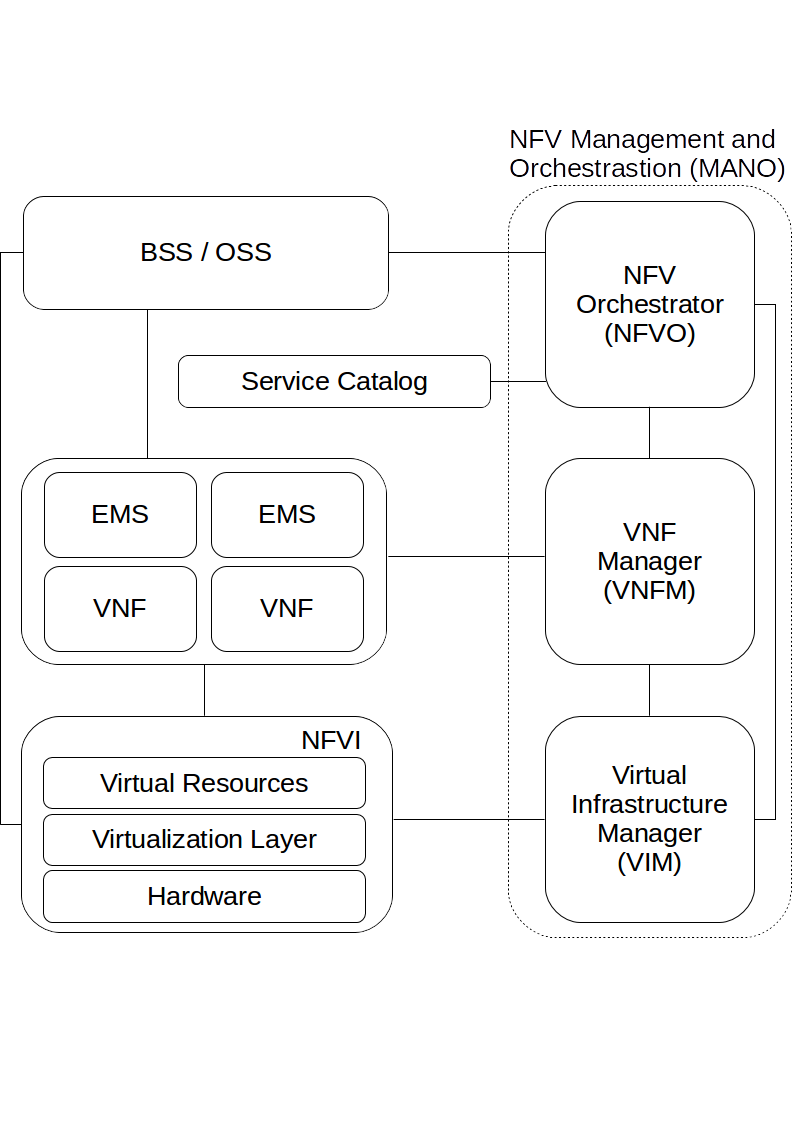
\includegraphics[]{mano.png}
\caption{ETSI NFV Architecture}
\label{fig:mano}
\end{figure}

\subsection{Architecture}
\subsubsection{Network Function Virtualization Infrastructure (NFVI)}
Network function virtualization infrastructure block of the ETSI NFV model that provides the necessary
environment for virtual network functions. It consists of three parts. The first is the physical hardware
that will provide the essential resources like processing power, storage and networking etc. They are
assumed to be commercial off the self hardware. The second is the virtualization layer that will enable
virtual network functions to use underlying architecture. As long it supports the use required reference
points ETSI model doesn't require any specific virtualization solution. The third one
are the pooled virtual resources will then be exposed for the use of upper levels.

\subsubsection{Virtualized Network Function (VNF)}
A virtualized network function is a virtualization of the existing network functions that are often
implemented as specialized hardware. VNFs are expected to function identically compared to their non 
virtualized counterparts. It is not necessary for a single VNF to be implemented in a single virtual
machine. Implementation details may depend for the nature of the network function.

\subsubsection{Element Management System (EMS)}
Element management system is a functional block that will handle the management tasks for one or
multiple VNFs. This management tasks include fault management, accounting, configuration (could be 
vendor specific configuration), security and performance evaluation. The EMS may or may not collaborate
with the virtual network function manager.

\subsubsection{Operations Support System / Business Support System (OSS/BSS)}
Operations Support System/Business Support System block is reserved for the network
operators. They can define any operation that are not explicitly described in the core
ETSI architecture. It is expected to share data with other function blocks.

\subsubsection{Virtualized infrastructure manager (VIM)}
Virtualized infrastructure manager block is responsible from the management of the network function
virtualization infrastructure. Mainly VIM has to orchestrate NFVI resources. For this VIM has to make
an inventory of system resource, keep track of what resources available at any time, know how currently
allocated resources are utilized, is there any apparent hardware failures etc.
A NFV architecture can have multiple VIMs and there can be different VIMs for different resources in 
the NFVI. Openstack is a usual practical choice as virtualized infrastructure manager for the majority
of the ETSI NFV implementations.

\subsubsection{VNF Manager (VNFM)}
VNF Manager block is the software that manages the life cycles of the virtual network functions. Life
cycle of a VNF includes instantiation (mostly from a template and template generally includes
configuration information), modification, termination, monitoring, measuring performance metrics,
disaster recovery etc. VNFM generally implements VNF life cycle as a set of general commands that can
be applied almost any VNF regardless of type and each VNF in the system is assigned to a VNFM.
Likewise in VIM there is no limitation of how many VNFMs can exist together.

\subsubsection{NFV Orchestrator (NFVO)}
NFV Orchestrator is responsible for both orchestrating NFVI resources over multiple VIMs and managing
network services' life cycle. A network service is an abstraction for multiple virtual or physical
network functions and any service chains or forwarding graphs that interconnects them. A network
services' live-cycle is alike to a virtual network function and consists of instantiation (with
coordination the VNFM), modification, termination, monitoring, measuring performance metrics, disaster
recovery etc. Other duties of an includes keeping a catalog of existing network services and virtual
network functions, on-boarding new services, managing VNFMs etc.

\subsection{Implementation: Openstack Tacker}
In NFV MANO implementations Openstack is one of the most commonly used VIMs. To have a complete MANO
solution Openstack started a NFVO-NFVM project called Tacker. It's a spin-off of a Neutron project
called ServiceVM started in 2014 to provide a unified interface for life-cycles of different
appliances. While not successful as a Neutron project it evolved to implementing MANO in Openstack.
Since 2015 Tacker project exists as an NFV MANO solution in Openstack.

Tacker has a modular architecture that allows using it use with various different kinds of
existing Openstack services like Openstack orchestration service Heat and Openstack monitoring service
Ceilometer. VNF definitions (VNFDs) are described as TOSCA templates and saved in a service catalog.
Operators can also configure and monitor the VNFs by their requirements by writing custom management or
monitoring drivers.

Tacker uses TOSCA YAML templates for its virtual network function definitions. TOSCA or Topology and
Orchestration Specification for Cloud Applications is a format for defining applications that are needed
to run on a cloud architecture. The specification is developed by an non-profit standards organization
called Organization for the Advancement of Structured Information Standards (OASIS).
A TOSCA template defines not only application that user wants to deploy but also
it's requirements and the infrastructure it will run on. The main method of achieving
this feat is by defining relations between these units.

%\section{Service Function Chaining}

\chapter{Container Virtualization}
\section{Introduction}
National Institute of Standards and Technology defines cloud computing as a model for enabling
easy access to a pool of computing resources that requires minimal intervention from the service
provider. With cloud services, any person or organization can buy computing resources from providers
without the need of investing in computing infrastructure themselves. 

One of the essential technologies for implementing cloud services is virtualization. In modern cloud
environments the usually preferred method for virtualization is called hypervisor based virtualization.
Xen and KVM can be called the two most common free and open source hypervisors. While Xen is used in
biggest public cloud platform Amazon Web Services, KVM is used in Google Cloud Platform and Openstack.

The main goal for the hypervisors is to isolate virtual machines in physical host to a degree that they
are no different than separate computers in a network. Virtual machines run a separate operating system
called guest operating system and hypervisor mediates the system calls to the host operating system.
This technique is very efficient at isolating virtual machines but it also introduces an overhead
since there is an extra layer of abstraction. Previous studies show that while CPU and memory overhead
is minimal, biggest overheads occur in I/O operations. There is also some operational overheads that
comes from running an separate full-fledged guest OS. It also needs to be maintained and updated.

Recently there is another method of virtualization gaining traction in both research and the industry.
It's called operating system level virtualization or more commonly container virtualization.With
container virtualization virtual machines or containers have their own process and resource space but
they use host machines kernel and resources directly. Without the need of complete isolation and an
unaware guest OS container virtualization can achieve faster start up times, less resource consumption
and smaller images. But since all containers use the same kernel isolation between different containers
is weaker.

The earliest attempt for operating system level virtualization can be traced to the UNIX chmod command.
It is introduced in UNIX version 7 at year of 1979. By that time it could only provide file system
isolation. But FreeBSD jails is the first mechanism that can truly be called a container in a modern
sense. It was developed by Poul-Henning Kamp at 1998 and introduced in FreeBSD version 4 at 2000.
Jailed processed can't see other processes, can access only a specific part of their file systems and
have their own IP addresses. At Linux side, OpenVZ project developed a specialized kernel for running
containers at 2006. Contrary to jails, OpenVZ is more akin to a virtual machines. OpenVZ containers
have their own user structure, subject to configurable resource limits and can be migrated to separate
physical machines without the need of shutting down.

Despite both the concept and the technologies that make it possible were around for some time.
Containers are only recently started to see wide spread adoption. This can be explain with a couple
reasons. While Linux became one of the major platforms in the server domain there wasn't any container
technology available that can be run on an unmodified Linux kernel. Furthermore Linux kernel lacked
some of the essential capabilities to implement a container system such as resource management for
processes. Before cgroups was introduced in 2008 Linux kernel didn't have the capacity for controlling
and limiting the resources of a process or group of processes. Using cgroups and earlier introduced
kernel namespaces in the same year first native Linux
container project LXC was announced. While it didn't see much adopted by itself. It formed the basis
for the most of the modern container technologies.

\section{Docker}
Docker is a container virtualization technology that is developed in 2013 by a software company called
dotCloud. Among the modern container technologies Docker is the most widely used one and it would also
be fair to say Docker project's success is partially responsible for the recent adoption of container
virtualization technology. This might be attributed to Docker's different approach on how to prepare 
and use containers.

Virtual machines are used to be considered as virtual equivalents of physical dedicated servers and for
some time containers are also thought as faster and more lightweight virtual machines. But the main
contribution of Docker is focusing into an application instead of a server. Docker provides tools for
packaging an application and all of its dependencies together to run the application inside of a
container. This model of packaging and deployment of applications using containers also found out to be
a effective solution for an important problem at software development and maintenance. Because 
differences between development and production environments such as different operating systems, 
different versions of libraries and applications etc. is a common source for software bugs. Since they
are being used and  maintained by different people and there are no way any single person would be
aware of all the differences. Packaging the application and dependencies with Docker and running it in
containers prevents this problem. Because it guarantees the environment that runs in developer’s
machine and the production machine will be the same.

Furthermore Docker proposes that each component of an application should be run in a 
different container thus encouraging developers to use a loosely coupled software architecture that is 
also called micro service architecture. According to micro service architectures managing and updating
individual components of applications are easier compared to managing a monolithic application which
all of its components runs in same environments and problems in one component can affect the whole
application.

\subsection{Docker Images}
As mentioned before packaging the applications and dependencies together is one of the core ideas
behind Docker. This is achieved by using the Docker images. Contrary to virtual machines where user
has to install a new operating system on a clean virtual disk or use pre-installed disk image. Docker 
provides the tools to easily create new images from scratch or from existing images. Docker also
provides a central registry called Docker Hub where official and community created images can be found.
New images are created by using a template format called Dockerfiles.To create an image user has to
choose a base image and then has to describe what changes has to be made on this base image with
provided commands. An example Dockerfile can be found at the appendix. Then using the Docker build
command will create the intended image.

Docker images are declarative constructs. An existing Docker image can not be edited or changed. This
way it's guaranteed to have the same environment every time an image is used. To make changes to an
image a new image has to be created. Docker has a version control system for images and a new version
of the image doesn't have to overwrite the old images. This way in case of errors and failures old
versions can still be used. Since storing whole copies of all images would take too much disk space.
Docker uses a different storage technologies for storing images.

Docker images are stored using a storage model called union file systems to minimize storing duplicate
data. Using this model images are consisted of several ordered layers. Each layer has it's own file
system and if a file is present in multiple layers only the file on the top most layer is visible. When
creating a new image Docker takes all the layers from the base image and adds new layer or layers
according to the Dockerfile. If we make create a new version of a image only the changes are also 
written to a new layer. Normally layers are read only file systems but since container that can not
write data to their disks would be unusable a writable layer is added when a container is created. This
layer would be deleted when the container is removed until it's saved as a version of the image.
While Docker can use different union file systems, by default AUFS is used.

\subsection{Architecture}
Docker uses a rather simple server-client architecture for the creation and management of the
containers. The main components can be summarized as the Docker engine, the component that manages
images and containers, Docker client, the component that users and administrators can send their
commands to Docker engine with and the Docker registry the component images that constitutes the core of
the containers resides. The communication between these components are achieved via REST APIs.

It's clear to see that the Docker engine is at the core of this architecture. It will be easier to
understand how the Docker Engine currently works if it's broken down to three sub components. The
container runtime is the component that runs the containers themselves. The container engine provides
the extra services that a container will need such as networking, storage, security etc. And The Docker 
services is the set of components that provides services that are crucial for Docker's internal
operation such as the Docker API, image management, authentication etc.

Docker's commitment to the above mentioned micro service architecture can also be seen in the evolution
of the Docker engine as it matures over time. Initially it was just a monolithic daemon. While it's
convenient to have a centralized system in the short run. In time the shortcomings of this model
started to appear and components started to become independent from the daemon. At first a plug-in
model developed to manage the aforementioned extra services. Then the container runtime was modified to
be able to run in a stand alone way. While the first container runtime for Docker was the LXC. It was
already replaced by a runtime called libcontainer which is developed by Docker themselves. The new
runtime that enabled libcontainer to be used without the docker daemon is called runC and it's managed
by a library called containerd. With this change docker daemon became a component that is only
connecting the API, service plugins and the containerd.

\section{Kubernetes}
The one of most important topics about operating cloud environments is the question of scale. In a
practical case it would be expected to run numerous amounts of containers in many hosts and since
cloud systems has to run with minimum human intervention. The obvious problem would be coordination
of the containers in a automated manner. The problem domain can be defined as container orchestration.
For container orchestration the main issues would be how containers will be distributed among hosts,
how they will communicate, what happens when the containers fail, what happens in case of on outage,
how will applications scale etc.

Kubernetes is a container orchestration software that is developed by Google in 2014. It's design is
inspired by Google's internal container orchestration systems Borg and Omega. Kubernetes is a free and
open source software and it's ownership is later transfered to a more neutral organization Cloud Native
Computing Foundation that is run by Linux Foundation. Kubernetes is written in Go programming language.
It can be installed into physical servers, local virtual machines or public cloud services. Although
Docker now has it's own integrated container orchestration solution called Docker Swarm, Kubernetes
stays as the most widely used container orchestration software.

\subsection{Architecture}
Kubernetes implements a typical master slave architecture. These are named as master nodes and worker
nodes. Each of these nodes has to run several Kubernetes components according to their roles in the
cluster. For master nodes the required components are API server, etcd, scheduler and
controller manager, for worker nodes the required components are kubelet and proxy. A representation
of Kubernetes architecture can be seen at Figure \ref{fig:k8sarch}

\begin{figure}
\centering
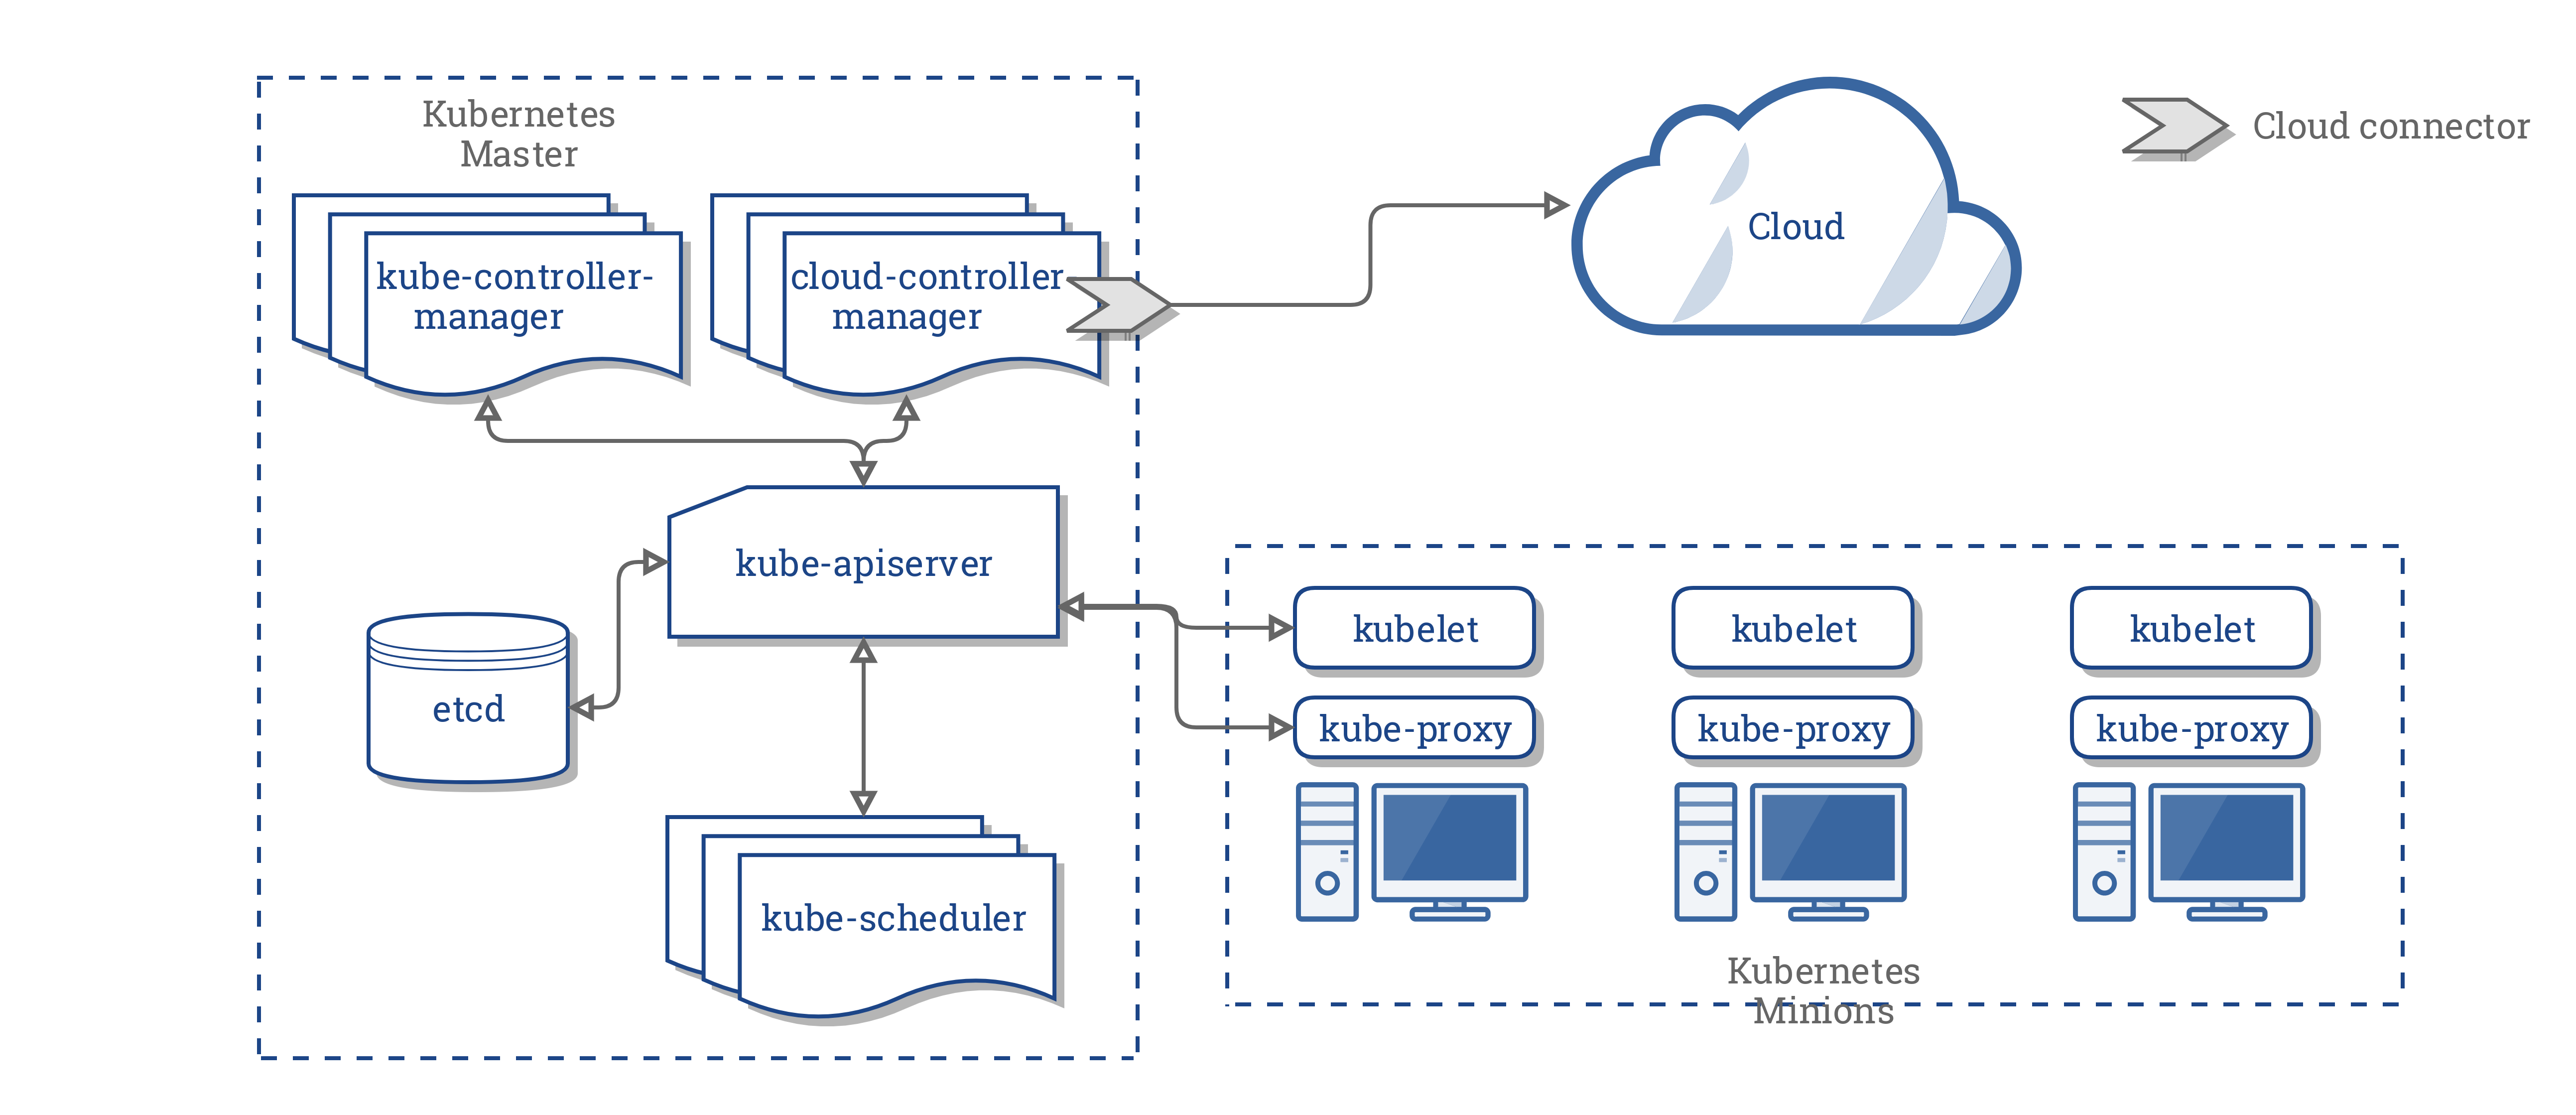
\includegraphics[]{k8s-arch.png}
\caption{Kubernetes Architecture}
\label{fig:k8sarch}
\end{figure}

API server is the component that serves the Kubernetes API. The entire control plane of Kubernetes is
built on the API and components doesn't have any other way to communicate with each other. API server
is designed to be stateless and all the necessary data is stored on etcd.
Etcd is a distributed key value store that is developed by CoreOS. It serves as a central database for
the Kubernetes cluster. Since etcd stores the whole cluster state, consistency and fault tolerance is
critical. It uses a consensus algorithm called raft to keep track of all the changes in etcd nodes.
Scheduler is responsible for assigning containers to appropriate worker nodes considering the resource
requirements, hardware conditions and several other factors.
Controller manager is a collection of software that watches the current cluster state and checks if it
matches with the records in the API such as node availability, current endpoints etc.
Kubelet is the main Kubernetes daemon in the worker nodes. Kubelet's main responsibilities are to 
manage containers and check both node's and container's current status and report it to the API.
Proxy is responsible from the networking in the worker nodes. It listens the API and configures the
node network accordingly so that containers can communicate without any problems.

Kubernetes used Docker as the main container runtime. To support different container runtimes kubelet
has to be modified significantly. Since it would be quite difficult for each runtime vendor to make
this modifications a common API is developed to easily integrate other runtimes into Kubernetes. This
API is called the Container Runtime Interface (CRI). While this is a relatively new technology,
introduced with Kubernetes version 1.5 there is some implementations using CRI such as CRI-O which
tries make Kubernetes compatible with Open Container Initiative runtimes and Rktlet a CRI
implementation of the CoreOS runtime rkt.

\subsection{Workloads}
For creating or accessing Kubernetes resources a developer first has to select an API client to work
with. It can be the web interface, one of the programming language clients or the kubectl command line
interface. Then they would need a definition of the resource or resources they want to create as an
Kubernetes API object. These object definitions or specs can be in JSON or YAML format and it would be
fair to liken them to orchestration templates. Kubernetes puts a special emphasis on associating the
objects. Associating your objects with meta data and using this meta data in other objects or
applications is one of the strong suits of Kubernetes specs.

The main unit of operation in Kubernetes is called a Pod. It can be seen as an abstraction of a single
application or a service. Pods are made from container or containers, IP address and if there is any
storage resources. Multiple containers within a Pod shares the Pod IP address and can communicate via
localhost. The namespaces and the IP address belongs to infrastructure container called, pause 
container and all other containers created runs as it’s children. so that failures among any of the 
pods containers don't affect each other and any of the containers can be safely restarted. It's 
recommended to only put applications that needs to be on the same namespace into a Pod together. This
includes the complimentary services such as logging, metric collection etc. Bundling application
containers and complimentary containers into a single pod also called the side car pattern. Pods are
considered temporary and disposable. They can’t heal themselves in case of failures and generally in
need of other structures for management like ReplicaSets and Deployments. These and a few other
constructs are called controllers.

ReplicaSets are a controller construct that can run any number copies of a Pod at the same time. A 
ReplicaSet will monitor the Pods and ensure that number of Pods designated in ReplicaSet definition are
running at any given time. It will spawn new Pods if some of current ones fail etc. ReplicaSets can
also be used for scaling. 

Developments are higher level controllers that also uses ReplicaSets for their operations. Main feature
of Deployments is to make updates to Pods easy and safe. They can progressively update the Pods they
monitor. Meaning it will spawn new Pods with updated image and terminate the Pods with old images as
the new ones becomes ready. In case of errors updates can be rollback to previous versions. Since
Deployments can do anything that ReplicaSets do and more. They are usually recommended over ReplicaSets
for general use.

There are also other controllers like DaemonSets which ensure copies of a Pod runs in every Node and
Jobs which are temporary Pods terminated after they completed their designated operation.

Since it’s expected from Pods to be disposable. It would not be reliable to try use Pod IPs for using
any service that a Pod provides. For example a front end shouldn’t have to track the ever changing IP
addresses of Pods that hosts it’s back end. Services are abstractions that provides reliable access to
Pods. The default behavior of services is to assign a virtual IP (called ClusterIP) inside a cluster
then forward traffic to this virtual IP to the Pods defined. Inside a node kube-proxy is responsible
from getting service definition from API and preparing forwarding rules generally using IP tables.
Beside using ClusterIP’s services can also define a port in each node for access called NodePort and
Services can also use load balancers if the infrastructure below supports it.
IP addresses of Services are only accessible from inside the cluster. For inbound connections to reach
any Service therefore any Pod there is a resource called Ingress. Ingresses are basically a set of rules
that forwards any inbound connection to any Service according to its definition. This definitions can
be IP addresses, domains and subdomains or paths to a domain. Besides creating an Ingress resource
users also have to create an Ingress controller. Ingress controller is actually a standard Pod that is
registered into controller list via the API. There are several alternatives for an Ingress controller,
Kubernetes project itself also provides an nginx based controller in their Github repository.

%\subsection{Networking}

\chapter{Experimentation}
\section{Setup}
This section will explain the test environments that all the experimentations will use. While this
setup has many components, all the software components are selected from available free and open source
tools.

The hardware used in this setup is a desktop computer. It's specifications are in the following
\begin{itemize}
 \item 8 core Intel i7-920 processor
 \item Asus P6T Motherboard
 \item 20 GiB 1066 Mhz DDR3 memory
 \item Ubuntu 16.04 64 bit operating system
\end{itemize}

One of most essential parts of this setup would be a cloud platform that can run and manage containers.
We chose the Kubernetes container orchestration software as a cloud platform after considering it's
features, widespread adoption and maturity. There is no standard way to setup a Kubernetes cluster.
While minikube can be used for development and testing purposes. It's method of creating a single node
cluster inside of a virtual machine would makes it unsuitable for mimicking actual clusters. Another
tool for building clusters by the Kubernetes team is kubeadm. Although it's currently on beta, it
allows easy installation among multiple nodes regardless of type. We selected kubeadm as the 
installation tool for our work. Installing kubeadm inside of Docker containers instead of virtual
machines we built a three machine Kubernetes cluster with one master and two nodes. This pattern is
often called dind or Docker in Docker. Kubeadm also leaves the network setup to the administrator's
choice via the CNI. Thus allowing us to experiment with different network configurations.

For monitoring the cluster state and container performance, an external tool is needed. As a monitoring
tool we chose Prometheus a modern pull based monitoring that is developed by the same non-profit that
also develops Kubernetes. Prometheus can be easily installed using the operator model. It can also
receive metrics from other applications via extensions called exporters. To use in the tests we also 
prepared a Docker image with a modified web server to be able send usage metrics to Prometheus. This
docker image contains a Nginx web server version 1.12.2 compiled with nginx-vts module.

\section{Experiment Design}
Before we start with experimenting with more advanced applications, it would be preferable to see this
setup's performance when a more typical application is used. We designed a preliminary experiment for
measuring network performance on Kubernetes using several different network setups.

As we mentioned before contrary to virtual machines, if they are not constrained containers have full
access to host machines computing resources and in a typical cloud environment we can assume that
containers will always run with constrained resources. Because of that will also constrain our
containers' resources. Until otherwise stated each pod will be constrained to 1/10th of a CPU core.

The test application will be a simple web server. It will be deployed to the cluster via Kubernetes
deployments using our Docker image. Kubernetes deployments are ideal deployment tools for this case 
because they can create and maintain a specified number of instances for an application and they also
can easily be scaled horizontally. We will create 3 separate deployments and for varying number of
instances in each deployment we will run series of tests simulating network traffic. For simulating
network traffic a http load testing tool bombardier will be used. It's a command line tool written in
Go programming language and it can save results in JSON format for easier further processing. All
containers inside a deployment will be exposed through single endpoints using Kubernetes NodePort 
services.

Our methodology for running the tests will be the following. 
\begin{enumerate}
 \item First we will choose a network setup and then create a Kubernetes cluster with 2 nodes.
 \item For each step we will create a pre-determined amount of instances for each deployment.
 \item For each deployment we will run the load test software to send various amount of requests from
 various amount of concurrent connections
\end{enumerate}

Number of instances used in the tests and parameters used for the load testing tools can be found below.

\begin{table}[h]
\caption{Web server load testing parameters}
\centering
\begin{tabular}{cc}
Connections & Total Requests\\
\specialrule{2pt}{1pt}{1pt}
20 & 10000 \\
40 & 30000 \\
60 & 50000 \\
80 & 80000 \\
100 & 100000 \\
\hline
\end{tabular}
\label{reqtable}
\end{table}

\begin{table}[h]
\caption{Number of instances for each deployment}
\centering
\begin{tabular}{ccc}
Deployment 1 & Deployment 2 & Deployment 3 \\
\specialrule{2pt}{1pt}{1pt}
1 & 1 & 1 \\
5 & 5 & 1 \\
10 & 1 & 1 \\
12 & 12 & 1 \\
25 & 1 & 1 \\
25 & 25 & 1 \\
37 & 37 & 1 \\
50 & 1 & 1 \\
50 & 50 & 1 \\
75 & 1 & 1 \\
100 & 1 & 1 \\
\hline
\end{tabular}
\label{instable}
\end{table}

The main motivation for selecting such an instance distribution can be explained with a few reasons.
First it will be desirable to learn how co-locating containers are affected if other containers sharing
the same host starts to experience heavy load. Second if multiple different services experience heavy
load how does this affect each other and other containers on the host. For this reasons we designed a
scheme that always have a control application that has a static instance count and instance counts of 
the other one or two application changes constantly.

\section{Results}
We executed the test set described above on three different Kubernetes networking plugins Calico,
Flannel and Weave. These plugins are selected because they are general purpose networks using
different architectures and we thought it would paint a accurate picture for Kubernetes networking
space. 

The experiment setup was run by automated scripts 10 times for each different cluster. The
results were then plotted using the arithmetic mean of the data collected from 10 experiments.

It can be seen for all cases even a ordinary desktop computer can run high number of container
instances. Even over 100 instances latency increase is very low. This suggests even this computer is
capable of running a higher number of containers. High latency is at the initial step is expected 
because only one container instance with constrained resources trying to respond to requests. But when
the instance count is increased latency improves linearly and upon reaching a point latency improvement
is flattened. There is slight increase at the final step because of the load increase of the host.
While the latency of each application increases greatly when both application experiences load this can
only be observed on the step two and not other steps. We can infer this is only caused by the lower
instance counts rather than any problems about co-location. Latency of the control application doesn't
seem to affected from the other applications' load, this fulfills one of important requirements for
network function virtualization.

While all three network plugins had very similar results. BGP based network solution Calico performed
marginally better compared to overlay based network solutions Flannel and Weave. 

\begin{figure}
\centering
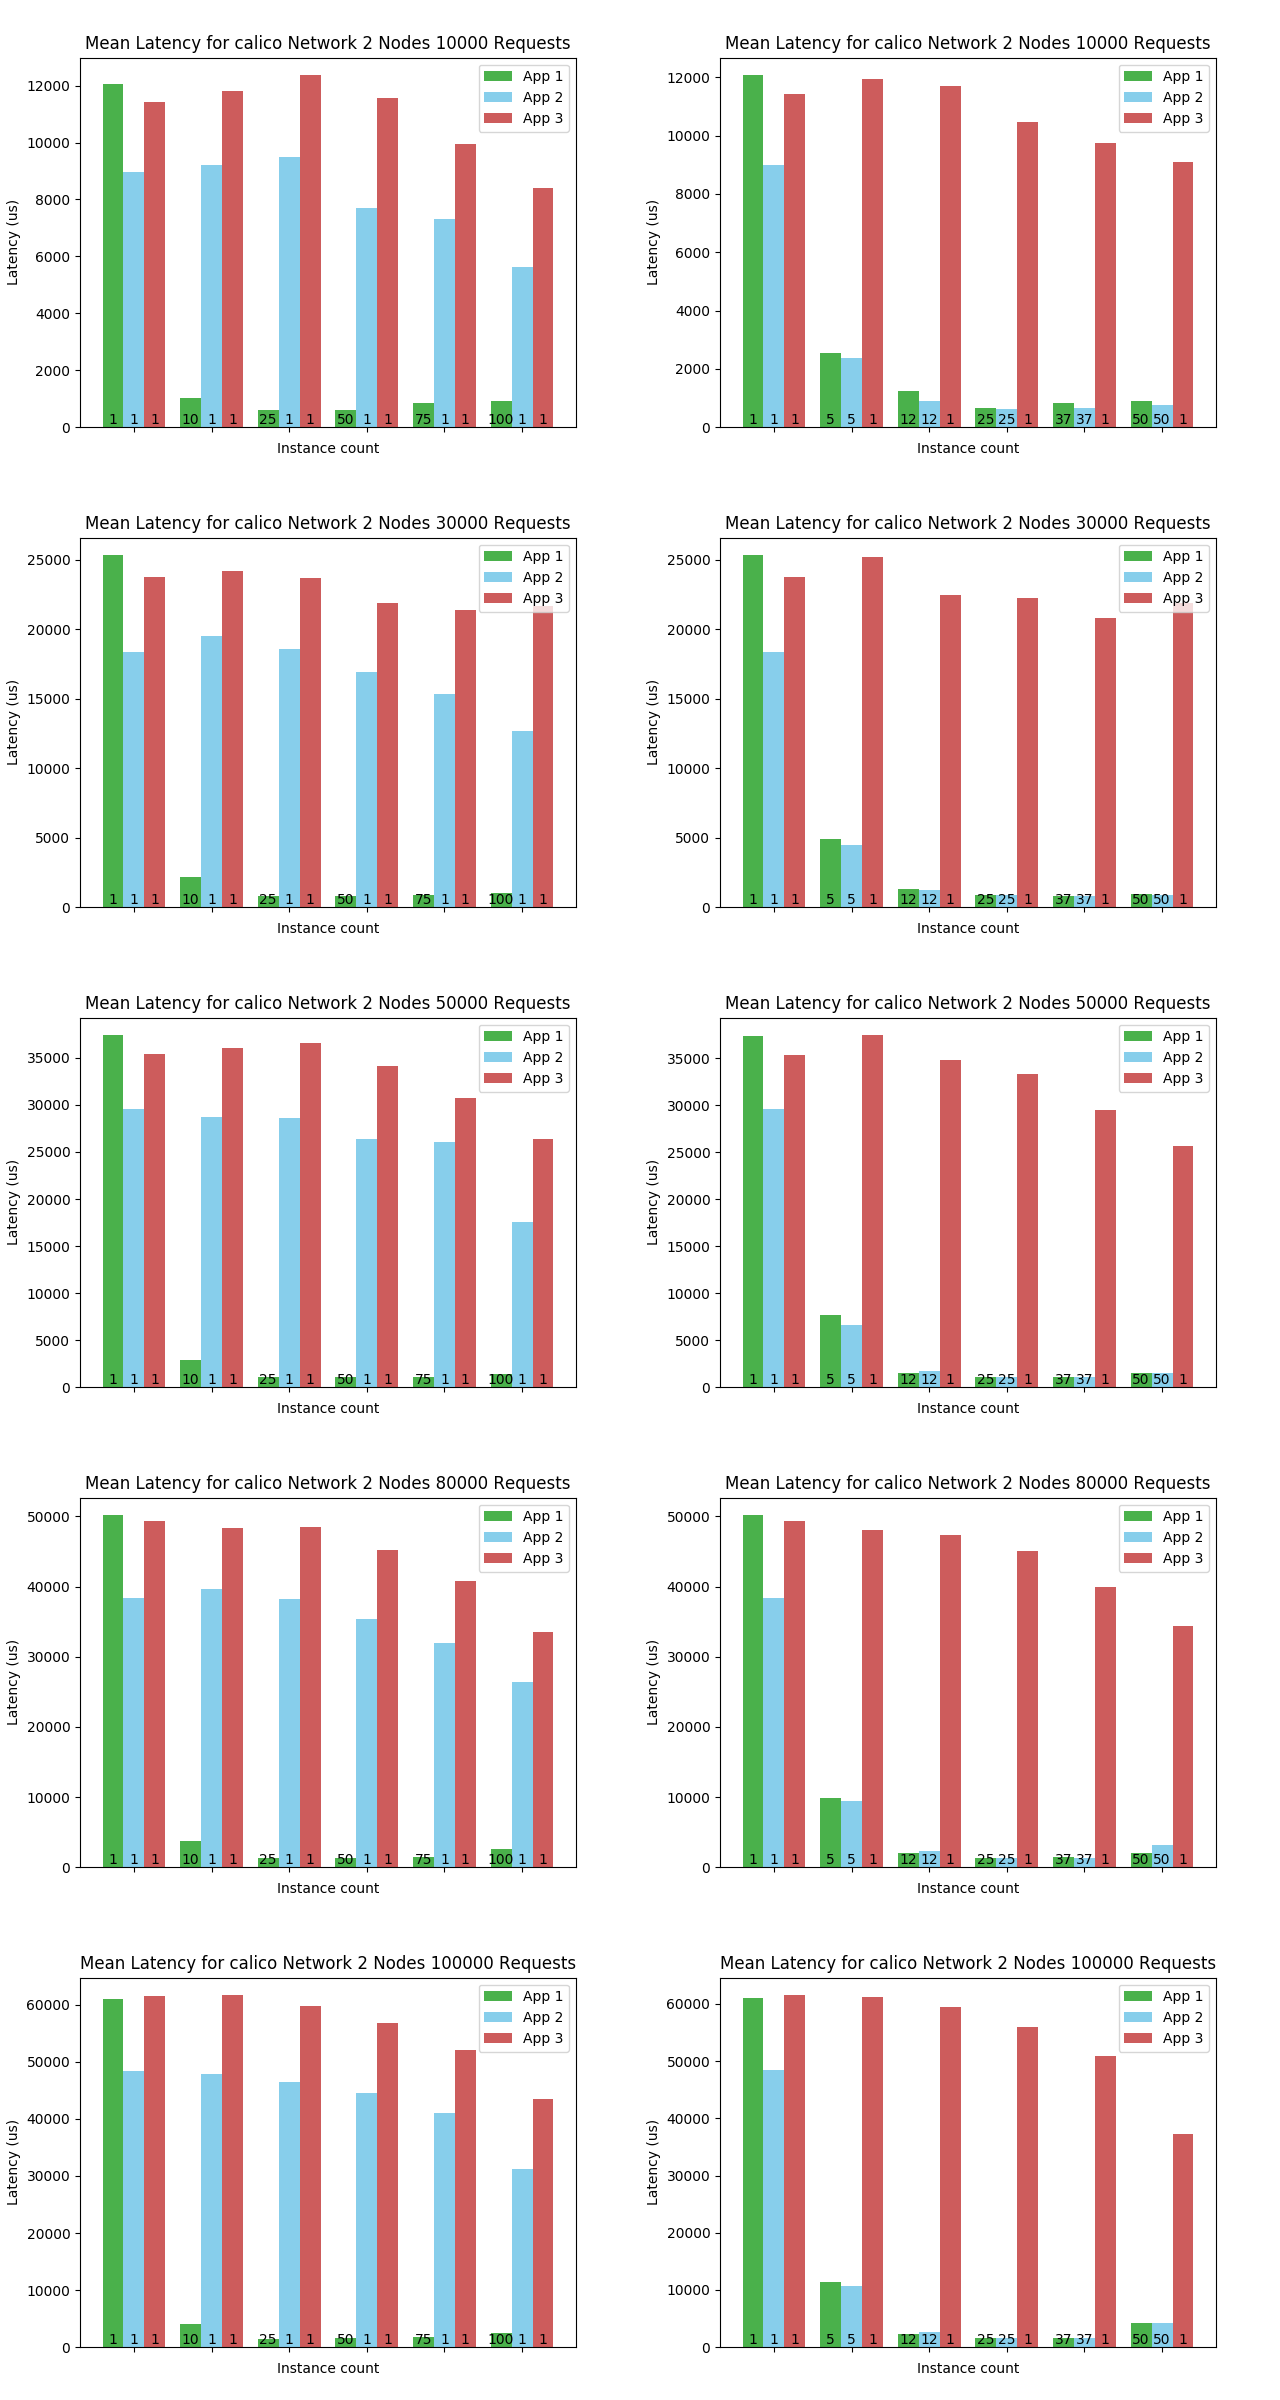
\includegraphics[]{calico.png}
\caption{Experimentation results for the cluster with Calico networking}
\label{calico}
\end{figure}
\begin{figure}
\centering
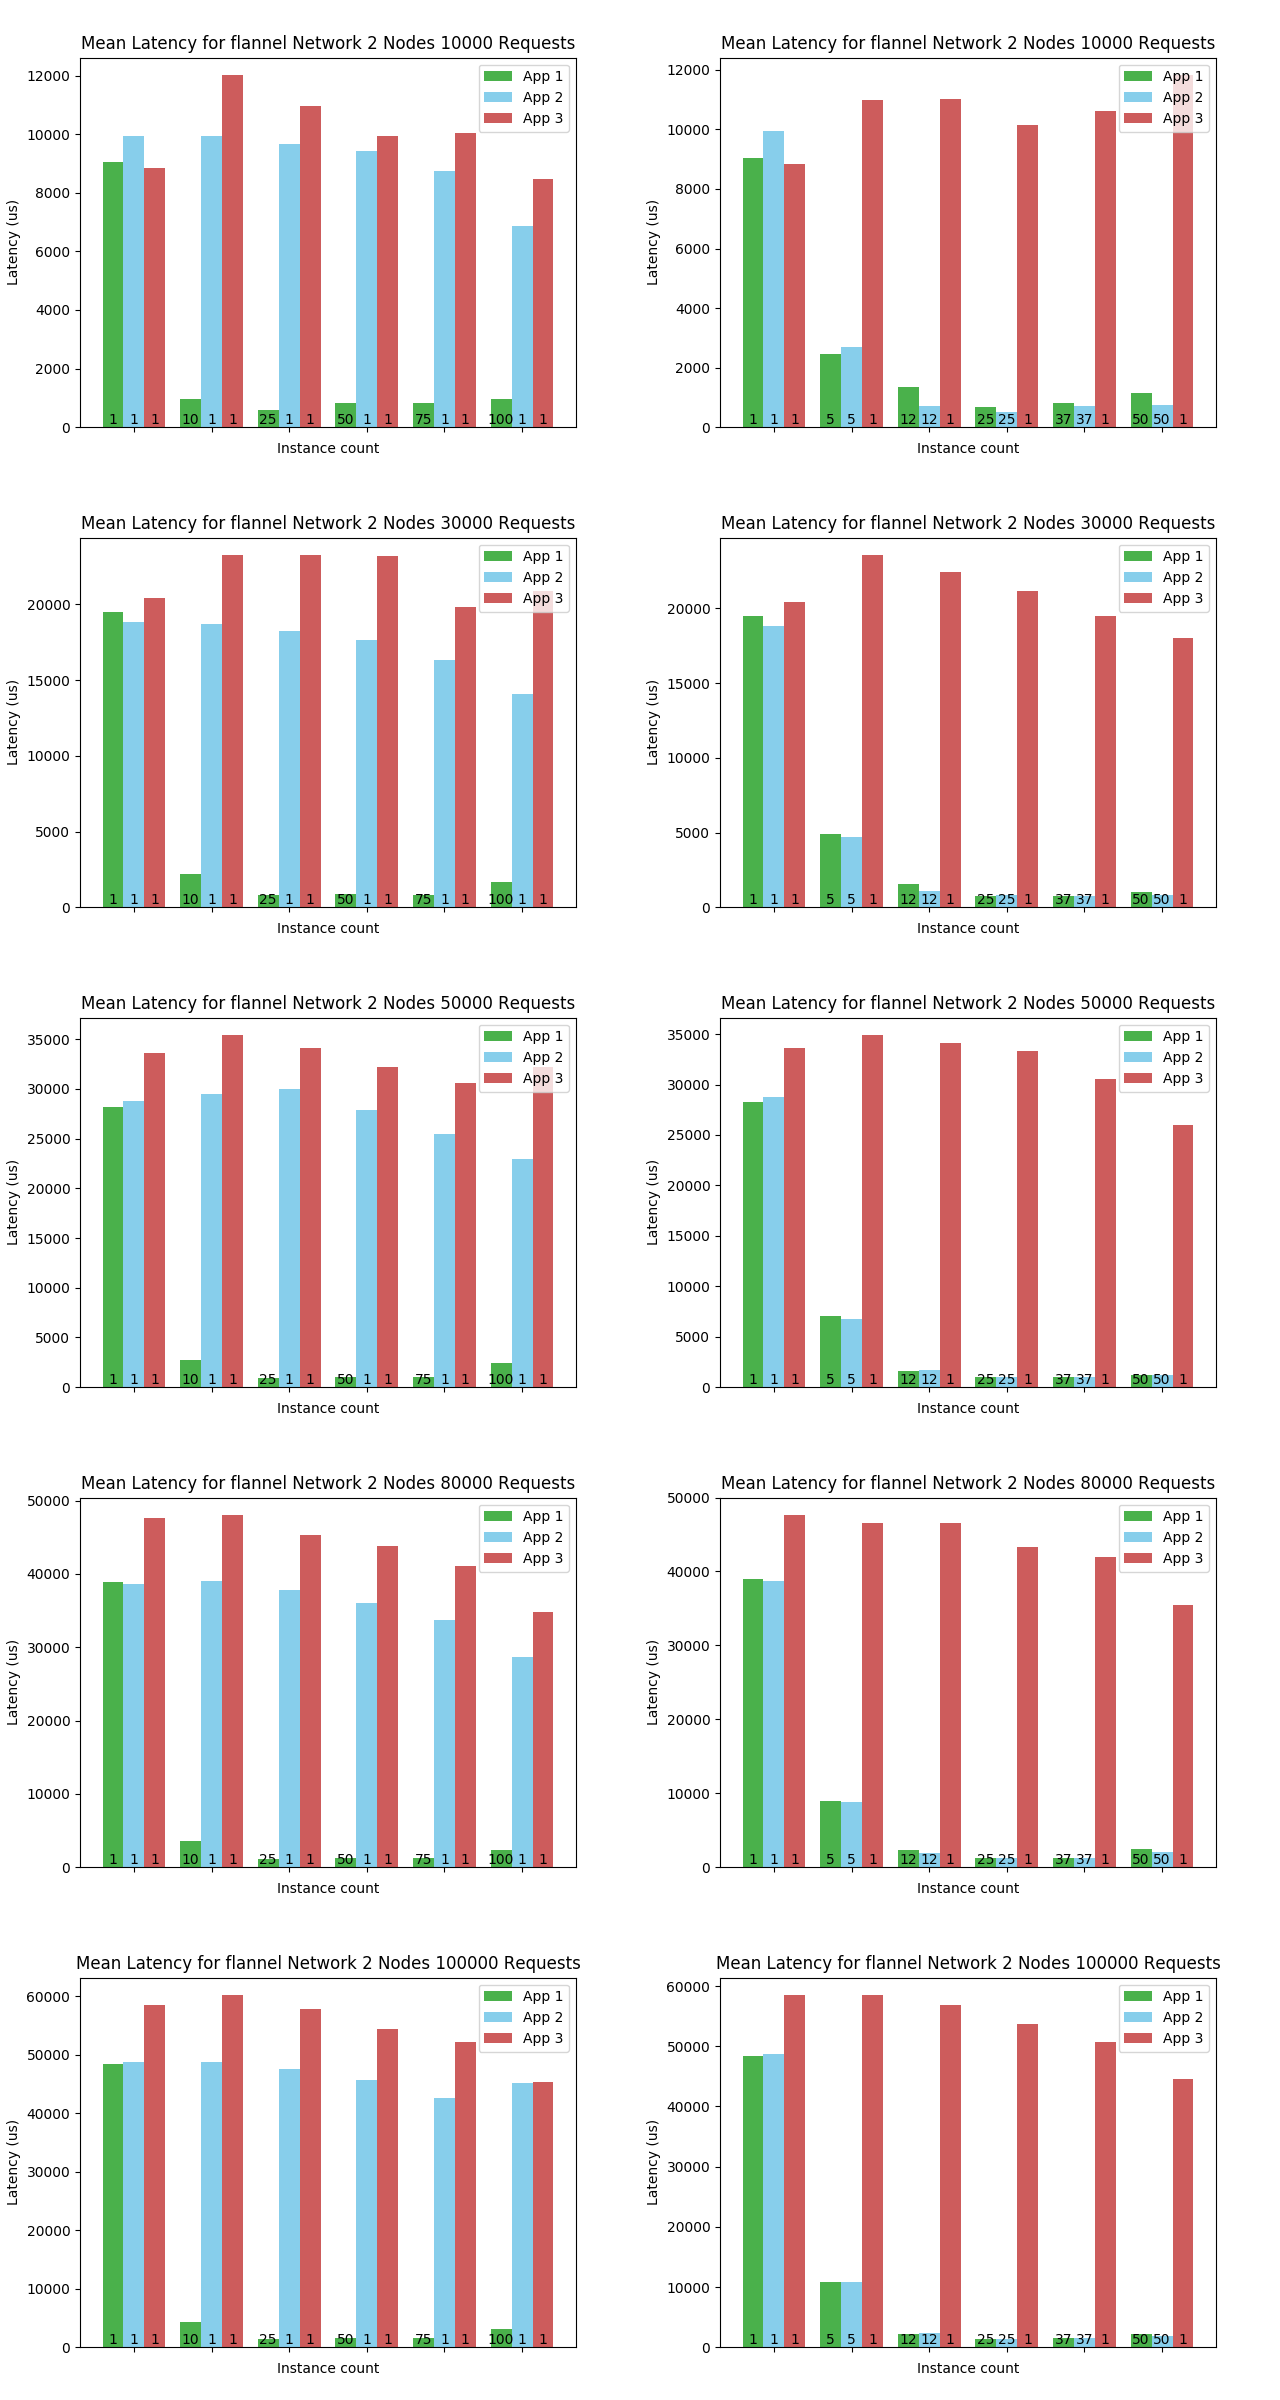
\includegraphics[]{flannel.png}
\caption{Experimentation results for the cluster with Flannel networking}
\label{flannel}
\end{figure}
\begin{figure}
\centering
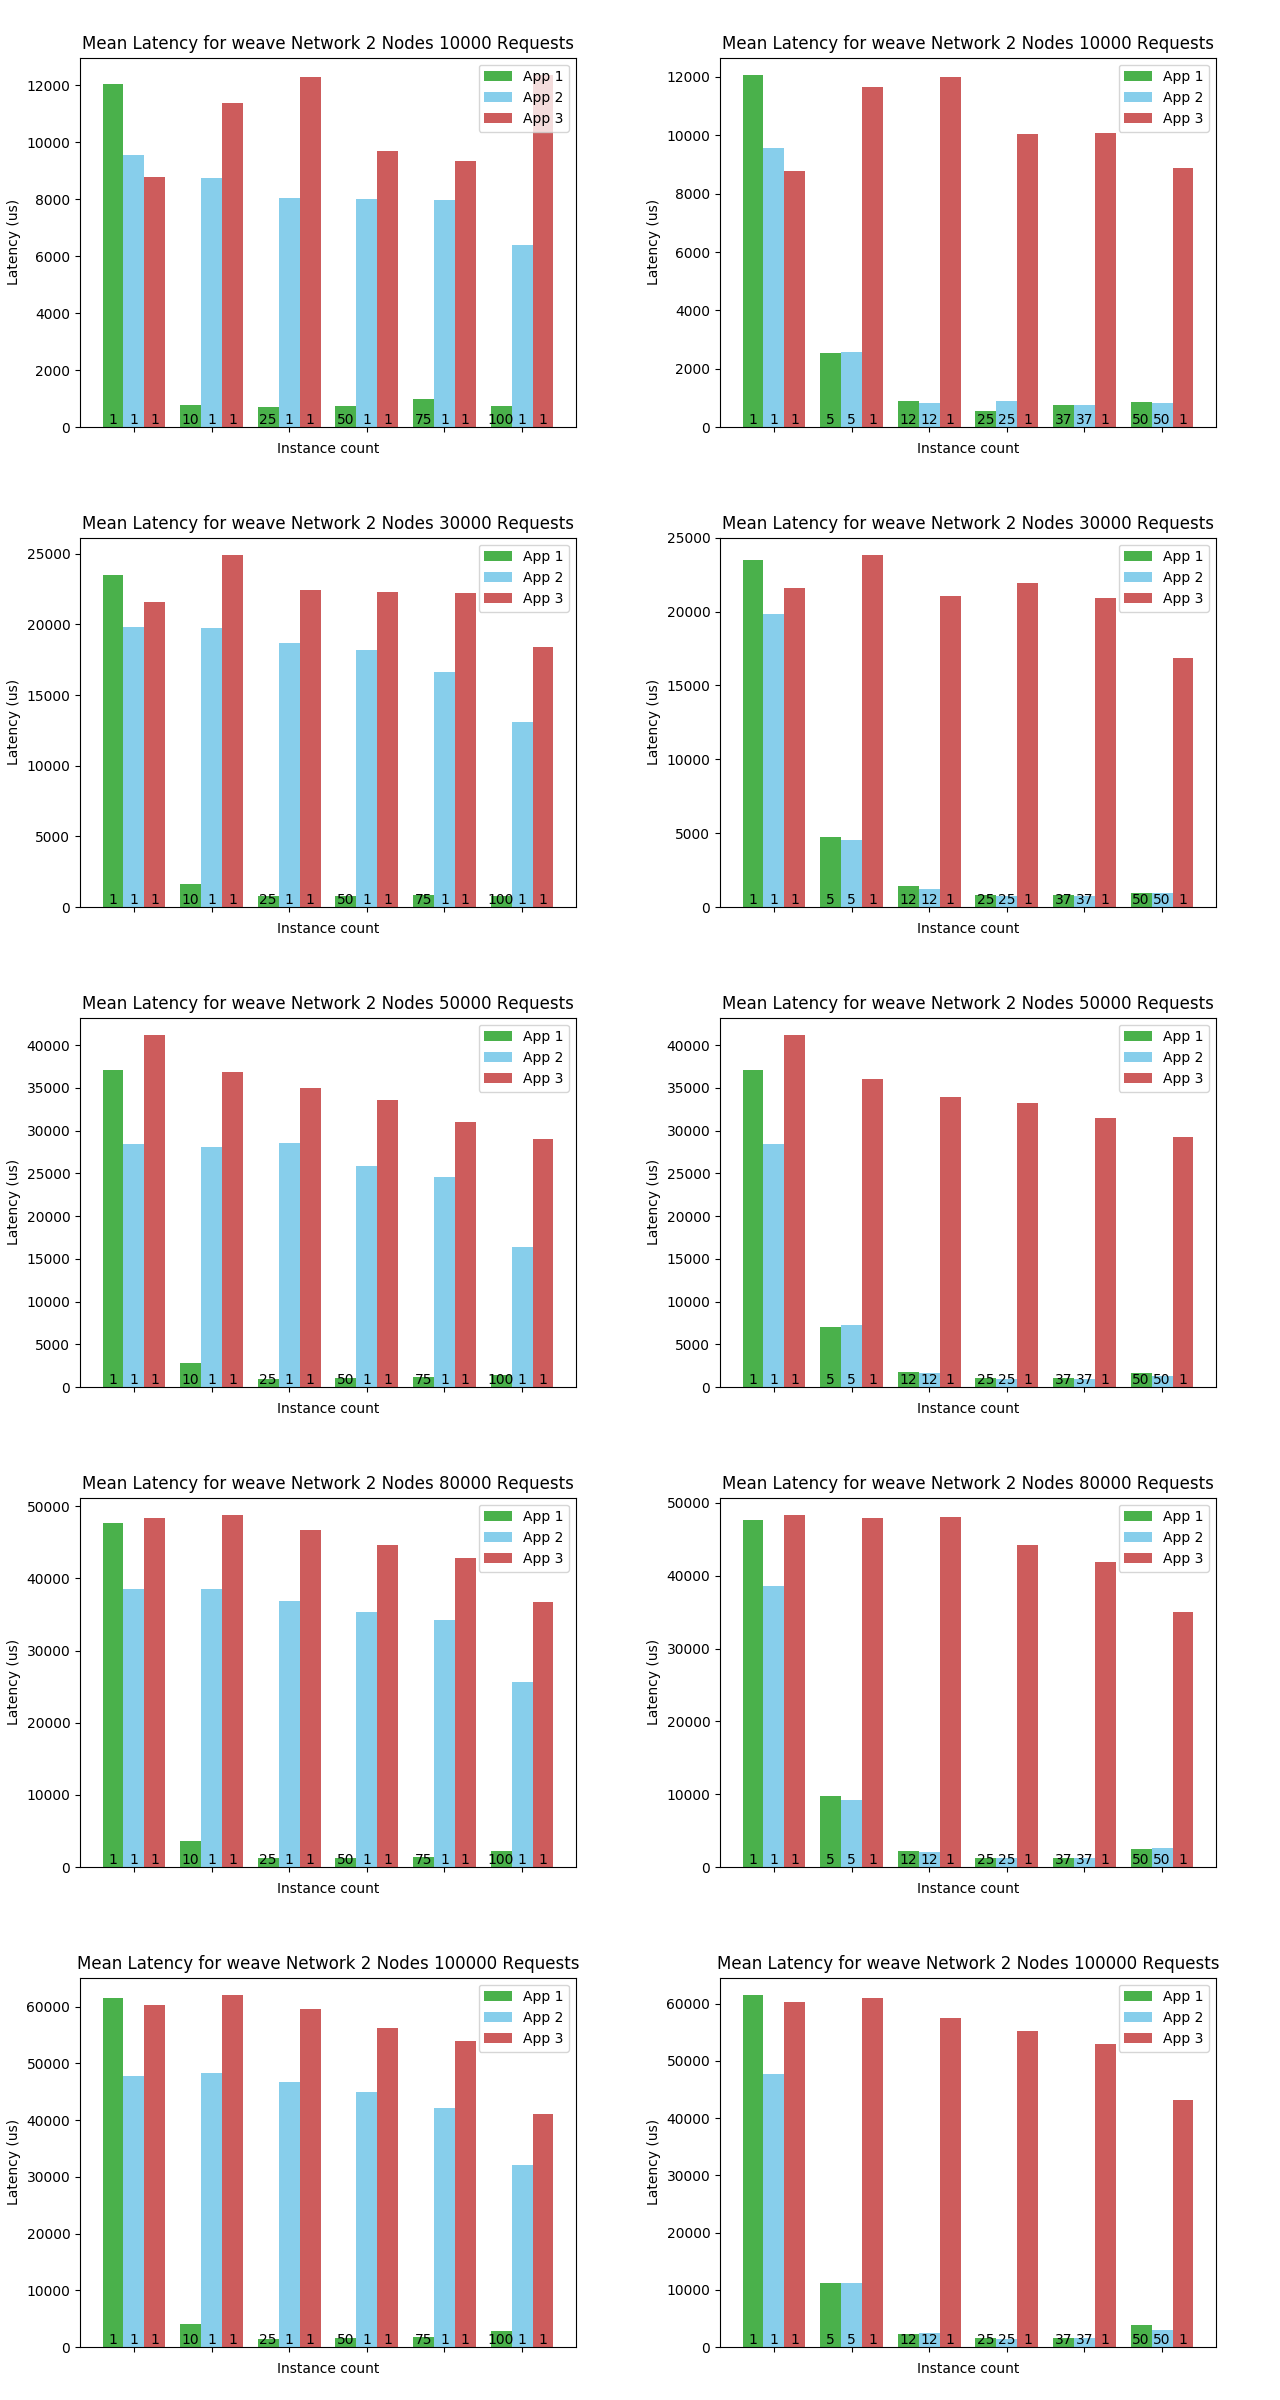
\includegraphics[]{weave.png}
\caption{Experimentation results for the cluster with Weave networking}
\label{weave}
\end{figure}

\chapter{Conclusion}
Virtualization is one of essential technologies behind modern computing infrastructure. In this work we
tried to examine to feasibility of combining two active subdomains of virtualization field. Network
function virtualization and container based virtualization.

At first we examined current systems for network function virtualization and tried to determine what
technologies are required to implement network functions, which architectures are preferred when
building systems to run network functions etc. Then we examined current container technologies and
tried to understand their capabilities, if there are alternatives or counterparts to technologies that
are required by virtual network functions.

We built a container testbed with Kubernetes for testing how containers perform under load and can they
adhere to often strict requirements for network functions. Our preliminary results show that the cases
that doesn't use specialized high speed networking software performed similarly regardless of which
networking setup was used. Results were varied between different experiments. Our conclusion was as is
standard container clusters can not be used for implementing virtual network functions.

But fundamental technologies that can used be for implementing virtual network functions in
container environments are present. Considering there is still no out of box solution exists these are
still immature and hard to install and use. We believe there are promising developments achieve network
function virtualization in containers. And in the future more practical solutions will be developed.

\section{Limitations and Future Work}
One of the main limitations of this work was the limited computing resources. Our testbeds was 
built into a common desktop computer. Which had very few resources compared to a common cloud
environment and this made it very hard to design a realistic system and limited the scale of our
experiments significantly.

For future work with a proof of concept MANO implementation for Kubernetes can be developed using high
performance networking software and other fundamental technologies required for network function
virtualization.

\appendix
\thispagestyle{empty}
%\chapter[]{Proof of Some Theorem}
%\thispagestyle{empty}
%This is appendix text.

%\curriculumvitae
\label{chapter:vita}
Uğurcan Ergün was born on June 19, 1991 in Istanbul. He graduated from Istanbul Köy Hizmetleri
Anatolian High School at 2009. He studied Computer Engineering in Kocaeli University and got his
Bachelor's Degree at 2013. In September 2013 he became a software developer for the Istanbul based
cloud service provider Skyatlas Inc. Since October 2015 he is a graduate student at Galatasaray
University.

%\section*{\uppercase{Publications}}
%\begin{itemize}
%\item If you have publications you must write there.
%\end{itemize}
%\thispagestyle{empty}

\end{document} 